
\section{Solving a Real Use Case: Functions of Two Variables}

In this tutorial, we assume that we have two functions for which we seek a
plot: the first is a sampled function given by a huge data file and the second
is the math expression $g(x,y)=\exp(-x^2-y^2)\cdot x$.

Our first function actually consists of two data files: the first file contains
some scattered data which resembles a discretization (``sampling'') of a
function and the second file contains data for the function as such, sampled on
a lattice. Our requirement here is two draw \emph{two} graphs into the same
axis: one in which the function is plotted as a smooth, colored surface and one
in which the scattered data file should be on top of the surface because it
provides more detail how the function was represented in the computer.

The second function which is given as math expression should be visualized
using a contour plot. A contour plot expects some fixed values $g_1, \dotsc,
g_k$ as input (the contour values) and plots one curve for each $g_j = g(x,y)$
(i.e.\@ if you go hiking without ever changing the height of your path).


\subsection{Surface Plot from Data File}

Our first step is to load the data file and to plot a surface.

Clearly, functions of two variables require a more sophisticated input format:
they are typically sampled on a unified grid with $n \times m$ points, i.e.\@
$n$~points for $x$ and $m$~points for $y$, resulting in a total of matrix with
$n\cdot m$ values $f_{ij} = f(x_i,y_i)$. How can we read matrix data? And what
if you have more than just the $z$ value? A standard way is to write the matrix
to a table, either in line by line ordering or in column by column ordering
(both are common).

Here, we assume that our function values are written to a table in which the
$y$ values vary from line to line. Here is an extract of the data file (which
is too large to list it here):

    \lstinputlisting[
        columns=fixed,
        breaklines=false,
        firstline=1,
        tabsize=15,
        lastline=6,
    ]{plotdata/concat_VV_together.dat}%
        \vskip-0.9\baselineskip
            $\vdots$
        \vskip-0.4\baselineskip
    \lstinputlisting[
        columns=fixed,
        breaklines=false,
        firstline=34,
        tabsize=15,
        lastline=43,
    ]{plotdata/concat_VV_together.dat}%
        \vskip-0.9\baselineskip
            $\vdots$

Note that the data file (and all others referenced in this manual) are shipped
with \PGFPlots{}; you can find them in the subfolder
\texttt{doc/latex/pgfplots/plotdata}.

The input file contains $x_0$, $x_1$, and $f(x_0,x_1)$ in columns named |x_0|,
|x_1|, and |f(x)|, respectively. In addition, it contains some meta data which
is irrelevant for us here.

Note that our input file contains \emph{empty lines} whenever |x_0| changes.
This is a common data format which simplifies the detection of ``scanline
length''. A scanline is one line in the input matrix, for example the line
consisting of all points with $x_0 = 0$. With such scanlines, \PGFPlots{} can
automatically deduce the size of the input matrix.

In order to plot the file as a surface, we proceed as in the previous example
by using |\addplot table|. However, we have to use |\addplot3| to indicate that
a three-dimensional result is expected: \pgfplotsexpensiveexample
%
\begin{codeexample}[]
\begin{tikzpicture}
\begin{axis}
    \addplot3 [
        surf,
        mesh/ordering=y varies,
    ] table {concat_VV_together.dat};
\end{axis}
\end{tikzpicture}
\end{codeexample}
%
The example looks familiar compared to our results of the preceding tutorials:
a |tikzpicture| environment containing an |axis| environment and the mentioned
|\addplot3| command. The option list contains |surf|, which tells \PGFPlots{}
how to visualize the input data. The key |mesh/ordering=y varies| tells
\PGFPlots{} how to decode the input matrix. This is important; otherwise
\PGFPlots{} would have chosen |x varies| which does not match our file.

Note that we there is no need to configure either |mesh/rows=|\meta{N} or
|mesh/cols=|\meta{N} here because these parameters are automatically deduced
from the scan line lengths marked by empty lines in our input file.

Since our |\addplot3 table| statement does not contain any hints which columns
should be plotted, \PGFPlots{} simply plots the first three columns against
each other.

The colors of a |surf| plot are chosen from the function values (unless you
configure some other value for |point meta|; this is similar to the scatter
plot example). In case of a function of two variables, the function value is
the third column.


\subsection{Fine-Tuning}

In order to stress how colors are to be mapped to values, we add a color bar to
our example from the previous subsection. In addition, we rotate the view a
little bit and add axis labels. Furthermore, we would like to have a smooth
color mapping.

We end up at
%
\pgfplotsexpensiveexample
\begin{codeexample}[]
\begin{tikzpicture}
\begin{axis}[
    view/h=40,
    colorbar horizontal,
    xlabel=$x$, ylabel=$y$,
]
    \addplot3 [
        surf,
        mesh/ordering=y varies,
        shader=interp,
    ] table {concat_VV_together.dat};
\end{axis}
\end{tikzpicture}
\end{codeexample}
%
Here, |view/h| rotates the ``horizontal'' parts of the view (only). It chooses
a new view angle for the orthographic projection. As you guessed, there is also
a |view/v| key and a |view=|\marg{h}\marg{v} variant.

The key |colorbar horizontal| is a style which activates a |colorbar| and
configures it to be displayed horizontally. The labels are placed using
|xlabel| and |ylabel| as we saw it before for visualizations of one-dimensional
functions. A colorbar uses the current |colormap| and adds axis descriptions to
show how values are mapped to colors.

 The |shader=interp| key activates a smooth color interpolation.


\subsection{Adding Scattered Data on Top of the Surface}

As motivated earlier, we have a second data set, one which characterizes how
the function has been represented in some computer simulation. We would like to
add the second data set as scatter plot on top of the function.

The data set as such is the very same as the one used in
Section~\ref{sec:tut3:usecaseA}, so we do not need to list it here again.
However, we have to include the two-dimensional scatter data into the
three-dimensional axis in a suitable way. We chose to place it on a fixed $z$
value as follows:
%
\pgfplotsexpensiveexample
\begin{codeexample}[]
\begin{tikzpicture}
\begin{axis}[
    view/h=40,
    colorbar horizontal,
    xlabel=$x$, ylabel=$y$,
]
    \addplot3 [surf,mesh/ordering=y varies,
        shader=interp
    ] table {concat_VV_together.dat};

    \addplot3 [blue,mark=*,
        mark options={fill=blue!80!black},
        only marks,mark size=0.6pt,
    ] table [z expr=1.2]{concat_VV_together_grid.dat};
\end{axis}
\end{tikzpicture}
\end{codeexample}
%
Now, we have two |\addplot3 table| statements in the same axis. None of them
uses the |cycle list| as we used explicit option lists. The first is our
surface plot. Note that it is plotted before the scatter plot: \PGFPlots{}
cannot handle depth information between adjacent |\addplot| statements. It
does, however, handle |z buffer| information for data of a single |\addplot|
statement. The second plot is our scatter plot: we recognize |only marks| and
|mark size| from Section~\ref{sec:tut3:usecaseA}. In addition, we configured
some color and marker options.

An important aspect is |\addplot3 table[z expr=1.2]| -- it tells \PGFPlots{}
how to choose $z$ values for the input file (otherwise, \PGFPlots{} would have
used the third column of that file). This is a convenient way to insert
two-dimensional data into a three-dimensional axis, provided you have
\emph{table} data. There is also a different way which works for both tables
and math expressions (or other input types). This different way is to install a
|z filter|, but that is beyond the scope of this tutorial for now.


\subsection{Computing a Contour Plot of a Math Expression}

This section addresses the second part of our use case example: a function of
two variables given by a math expression.

Our function of interest is $x \exp(-x^2-y^2)$. We start as in our tutorial for
one-dimensional functions given by a math expression (compare
Section~\ref{sec:tut1:step3}): by using an |\addplot| statement which is
followed by a math expression in curly braces. However, we rely on |\addplot3|
as in the preceding section:

\pgfplotsexpensiveexample
\begin{codeexample}[]
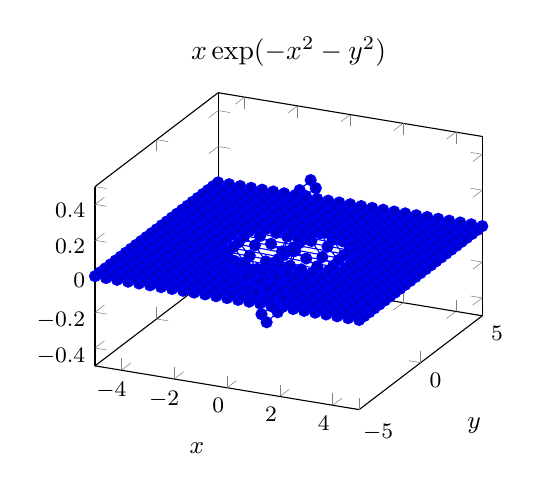
\begin{tikzpicture}
\begin{axis}[
    title={$x \exp(-x^2-y^2)$},
    xlabel=$x$, ylabel=$y$,
    small,
]
    \addplot3 {exp(-x^2-y^2)*x};
\end{axis}
\end{tikzpicture}
\end{codeexample}
%
Our example contains a basic axis environment with |title|, |xlabel|, |ylabel|
and the |small| key which are already known from the preceding tutorials. The
|\addplot3| has no options and is immediately followed by the math expression.
The absence of options tells \PGFPlots{} to rely on its |cycle list|. This, in
turn configures |mark=*| with |blue| color -- and a line plot. A line plot
combined with |\addplot3| is of limited use; it merely connects all incoming
points. Since points are sampled as a matrix (line by line). Our next step will
be to define a suitable plot handler.

Note, however, that our math expression depends on |x| and |y|. These two
variables are the sampling variables of \PGFPlots{} in its default configures:
both are sampled in the |domain| of interest using the correct number of
|samples|. The |\addplot3| statement takes care of computing $N\cdot M$ points
in the correct sequence where $N$ is the number of |samples| for $x$ and $M$ is
|samples y|, the number of samples used for $y$.

We can see that our sampling |domain| is too large. Switching to a smaller
|domain| focusses on the interesting parts of our function:

\pgfplotsexpensiveexample
\begin{codeexample}[]
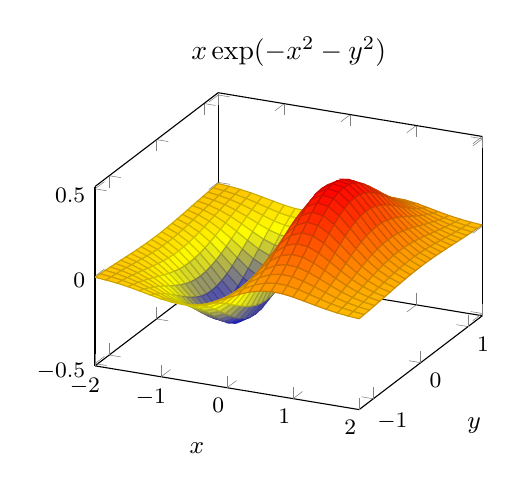
\begin{tikzpicture}
\begin{axis}[
    title={$x \exp(-x^2-y^2)$},
    xlabel=$x$, ylabel=$y$,
    small,
]
    \addplot3 [
        surf,
        domain=-2:2,
        domain y=-1.3:1.3,
    ] {exp(-x^2-y^2)*x};
\end{axis}
\end{tikzpicture}
\end{codeexample}
%
Here, we introduced an option list after |\addplot3|. Since we provided the
option list without the leading plus sign `|+|', \PGFPlots{} does not consider
its |cycle list| at all (and switches off |mark|s and the default color
settings). We added |domain| and |domain y| in order to restrict the sampling
domain in a suitable way. If we would have omitted |domain y|, the $y$ domain
would use the same value as the $x$ |domain|.

As you might have guessed, the |surf| key has the main use case of providing a
connection to the previous tutorial section: it is one of the natural
visualizations for functions of two variables. As in the preceding section, the
color has been deduced from the function value $z=f(x,y)$ (more precisely, by
relying on the default configuration |point meta=f(x)|).

The next step is to switch to contour plots by replacing `|surf|` by
`|contour lua|':

\pgfplotsexpensiveexample
\begin{codeexample}[]
\begin{tikzpicture}
\begin{axis}[
    title={$x \exp(-x^2-y^2)$},
    xlabel=$x$, ylabel=$y$,
    small,
]
    \addplot3 [
        contour lua,
        domain=-2:2,
        domain y=-1.3:1.3,
    ] {exp(-x^2-y^2)*x};
\end{axis}
\end{tikzpicture}
\end{codeexample}
%
Now, we have a contour plot -- although it is not quite what we had in mind.
First, there are so few contour lines that it is hard to see anything
(especially since the |line width| is too small). Furthermore, the |view|
direction is unfamiliar.

We add the |view| option with the argument for ``view from top'' and configure
the number of contour lines using the |contour/number| key and the |line width|
using the |thick| style:

\pgfplotsexpensiveexample
\begin{codeexample}[]
\begin{tikzpicture}
\begin{axis}[
    title={$x \exp(-x^2-y^2)$},
    enlarge x limits,
    view={0}{90},
    xlabel=$x$, ylabel=$y$,
    small,
	colorbar,
]
    \addplot3[
        domain=-2:2,
        domain y=-1.3:1.3,
        contour lua={number=14,labels=false},
        thick,
    ] {exp(-x^2-y^2)*x};
\end{axis}
\end{tikzpicture}
\end{codeexample}

This is what we wanted to achieve. Note that |contour lua| accepts options
which have the key prefix |contour/|. In this context, the prefix is optional.

Note that |contour lua| is different from almost all other plot handlers of
\PGFPlots{} with respect to one aspect: it requires you to invoke

|lualatex |\meta{texfilename}

\noindent instead of

|pdflatex |\meta{texfilename} .

\noindent 
The nonlinear algorithm to
compute contour lines is currently unavailable in plain \TeX{} which is stressed
by the name `|contour lua|'. 


If you cannot use |lualatex| for some reason, you can replace |contour lua| by |contour gnuplot|, provided that you have the external program |gnuplot| installed on your system (see the reference for |contour gnuplot| for more details).

\subsection{Summary}

We have sketched how to load a data table containing a sampled function of two
variables, and we learned how to visualize such data as |surf|ace plot. We
learned how to rotate the |view|, how to change the color |shader| of |surf|ace
plots, how to enabled |colorbar|s, and how to add |scatter| plots on top of
surface plots. Furthermore, we encountered the first contour plot as an example
for how to sample a function of two variables by means of built-in methods of
\PGFPlots{}.

It should be stressed that \PGFPlots{} needs no external tool to generate such
plots: every computer with a decent version of \PGFPlots{} can regenerate these plots.

There is more to say about three-dimensional axes, in particular regarding
|mesh/ordering|, parametric plots, perhaps line plots in three dimensions or
other plot types. Furthermore, there are some limitations regarding the
|z buffer|ing, i.e.\@ how \PGFPlots{} decides which parts of the figure are in
front of others. These items can be read in Section~\ref{sec:3d} and its
subsections.

You might also be interested in styles to change the appearance of a
three-dimensional axis, compare Section~\ref{sec:3d:axis:config}.
